\documentclass{article}
\usepackage{graphicx}
\usepackage[spanish,activeacute,es-tabla]{babel}
\usepackage[utf8]{inputenc} % mac utf8
\usepackage{amsfonts}
\usepackage{minted}
\usepackage{ucs}

\begin{document}

\title{\textit{Teoría de la Información y Codificación}\\ \textbf{Práctica 1: Creación código libre de prefijos con árboles binarios y cálculo de Kraft-Millan}}
\author{José A. Montenegro Montes}

\maketitle


\section{Enunciado}


La práctica  se centra en la construcción de códigos libre de prefijo utilizando un árbol, en este caso binario.
El usuario pasará los parámetros del código deseado y obtendremos una codificación si es posible.

\textbf{El alumno deberá realizar el método que realiza el cálculo de Kraft-McMillan} (KM) descrito en las transparencias del tema 2 (pagina 24). Verifique los resultados con el Ejercicio 7 (pagina 29) de las transparencias.

El número KM nos permite verificar si es posible crear un código libre de prefijos según unos parámetros datos. 

El objetivo principal que persigue la práctica es observar que mediante el calculo de Kraft-McMillan sabemos de antemano si se puede o no construir el código con los parámetros seleccionados, sin tener que calcularlos.
Observaremos el tiempo que tarda realizar el calculo con el árbol y el tiempo en calcular con Kraft-McMillan, tal y como muestra la figura \ref{fig:sistCom1}.

Tratando el tema de optimización observaremos que mediante una pequeña modificación en el cálculo de Kraft-McMillan (utilizando una alternativa a Math.pow) podemos bajar notablemente el tiempo empleado en su cálculo (figura \ref{fig:sistCom2}).
 

\begin{figure}[!hbtp]
\begin{center}
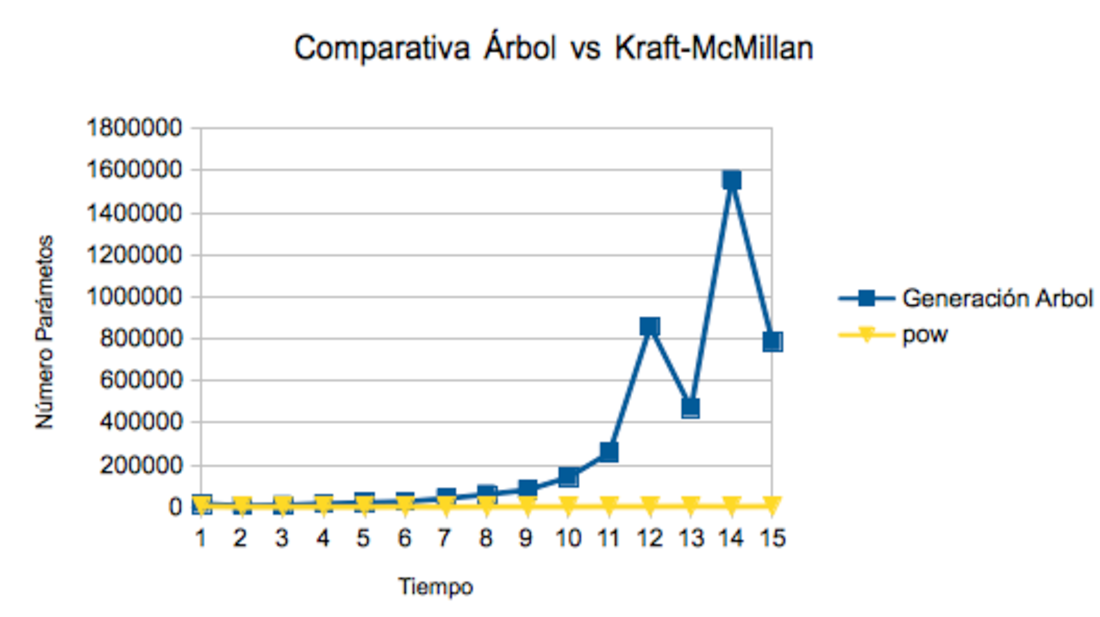
\includegraphics[scale=0.5]{ArbolvsKraftMcMillan.pdf}
\end{center}
\caption{Generación código Árbol vs Kraft-McMillan}\label{fig:sistCom1}
\end{figure}

\begin{figure}[!hbtp]
\begin{center}
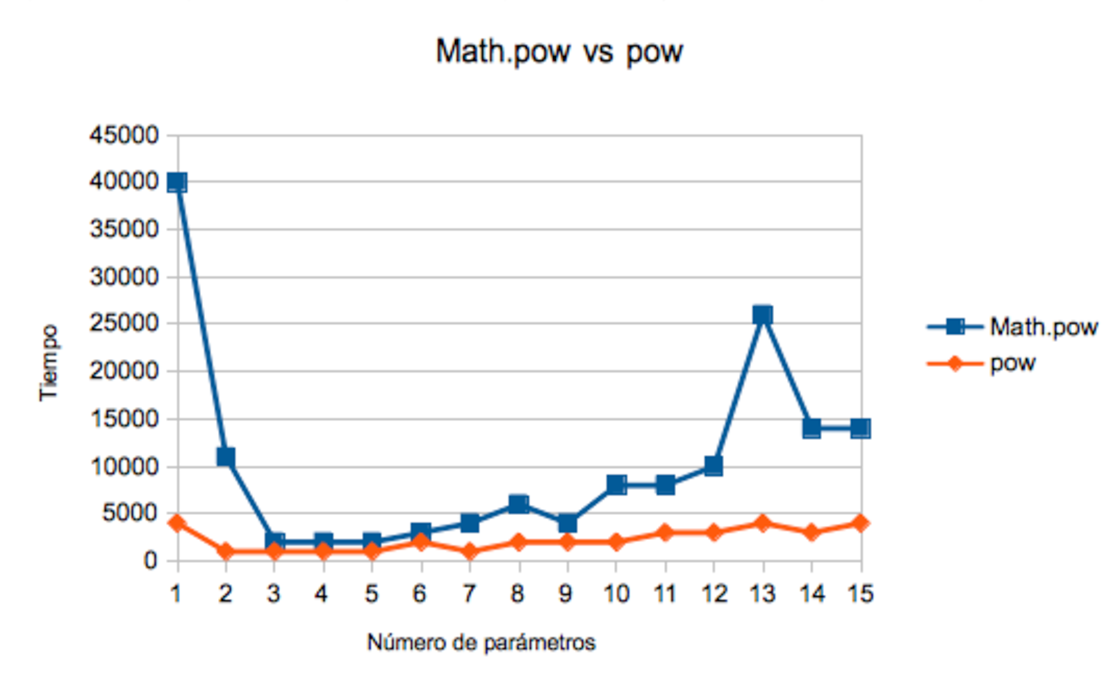
\includegraphics[scale=0.5]{GraficaMathVsPow.pdf}
\end{center}
\caption{Utilización Math.pow vs pow en Kraft-McMillan}\label{fig:sistCom2}
\end{figure}





\section{Conclusiones}

El objetivo de esta práctica es desarrollar código libres de prefijo mediante recorrido en un árbol binario, estructura que le resultará familiar al alumno.

Observaremos la utilidad de aplicar la fórmula de Kraft-McMillan para hacer más eficiente nuestro algoritmo.

Finalmente, veremos que aunque en la mayoría de los casos, es preferible utilizar la librería estándar de Java, en  ocasiones puntuales, una implementación propietaria puede mejorar los tiempos .



\section{Código}


\subsection*{Clase BinaryTreeCod } 

\inputminted[mathescape,
               numbersep=5pt,
               frame=lines,
               framesep=2mm]{java}{practica1/BinaryTreeCod.java}

               %%%%%%%%%%%%%%%%%%%%%%%
 
\subsection*{Clase TreeException Java.} 
\inputminted[mathescape,
               numbersep=5pt,
               frame=lines,
               framesep=2mm]{java}{practica1/TreeException.java}
               
%%%%%%



\end{document}
